\section{Exponential Functions}\label{sec:ExpFunctions}
An \dfont{exponential function} is a function of the form $f(x)=a^x$, where $a$ is a constant.
Examples are $2^x$, $10^x$ and $(1/2)^x$.
To more formally define the exponential function we look at various kinds of input values.

It is obvious
that $\ds a^5=a\cdot a\cdot a\cdot a\cdot a$ and $\ds a^3=a\cdot a\cdot a$, 
but when we consider an exponential function $\ds a^x$ we can't
be limited to substituting integers for $x$. What does $\ds a^{2.5}$ or
$a^{-1.3}$ or $\ds a^\pi$ mean? And is it really true that
$a^{2.5}a^{-1.3}=a^{2.5-1.3}$? The answer to the first question is
actually quite difficult, so we will evade it; the answer to the
second question is ``yes.''

We'll evade the full answer to the hard question, but we have to know
something about exponential functions. You need first to understand
that since it's not ``obvious'' what $\ds 2^x$ should mean, we are really
free to make it mean whatever we want, so long as we keep the behavior
that {\em is} obvious, namely, when $x$ is a positive integer.
What else do we want to be true about $\ds 2^x$? We
want the properties of the previous two paragraphs to be true for all
exponents: $\ds 2^x2^y=2^{x+y}$ and $\ds (2^x)^y=2^{xy}$.

After the positive integers, the next easiest
number to understand is 0: $\ds 2^0=1$. You have presumably learned this
fact in the past; why is it true?  It
is true precisely because we want $\ds 2^a2^b=2^{a+b}$ to be true about
the function $\ds 2^x$. We need it to be true that $\ds 2^02^x=2^{0+x}=2^x$,
and this only works if $\ds 2^0=1$. The same argument implies that $\ds a^0=1$
for any $a$.

The next easiest set of numbers to
understand is the negative integers: for example, $\ds 2^{-3}=1/2^3$. 
We know that whatever $\ds 2^{-3}$ means it must be
that $\ds 2^{-3}2^{3}=2^{-3+3}=2^0=1$, which means that $\ds 2^{-3}$ must be
$1/2^3$. In fact, by the same argument, once we know what $\ds 2^x$ means
for some value of $x$, $\ds 2^{-x}$ must be $\ds 1/2^{x}$ and more generally
$a^{-x}=1/a^x$.

Next, consider an exponent $1/q$, where $q$ is a positive integer. We
want it to be true that $\ds (2^x)^y=2^{xy}$, so $\ds
(2^{1/q})^q=2$. This means that $\ds 2^{1/q}$ is a $q$-th root of 2,
$\ds 2^{1/q}=\root q\of{2\ }$. This is all we need to understand that
$2^{p/q}=(2^{1/q})^p=(\root q\of{2\ })^p$ and
$a^{p/q}=(a^{1/q})^p=(\root q\of{a\ })^p$.

What's left is the hard part: what does $\ds 2^x$ mean when $x$ cannot be
written as a fraction, like $\ds x=\sqrt{2\ }$ or $\ds x=\pi$? What we know so
far is how to assign meaning to $\ds 2^x$ whenever $x=p/q$. If we were to
graph $a^x$ (for some $a>1$) at points $x=p/q$ then we'd see something like this:
$$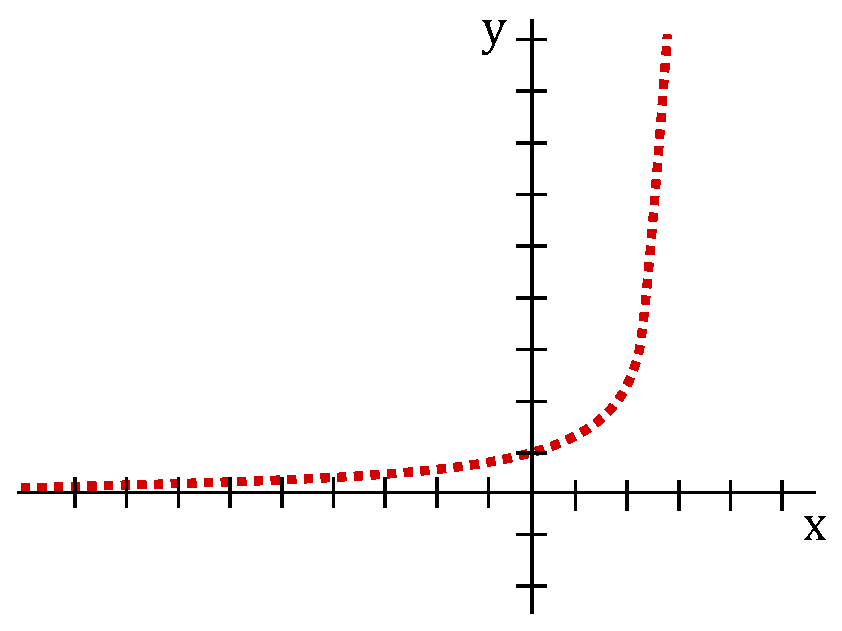
\includegraphics[width=2.5in]{images/exp1}$$

This is a poor picture, but it illustrates a series 
of individual points above the rational numbers
on the $x$-axis. There are really a lot of ``holes'' in the curve,
above $x=\pi$, for example. But (this is the hard part) it is possible
to prove that the holes can be ``filled in'', and that the resulting
function, called $\ds a^x$, really does have the properties we want,
namely that $\ds a^xa^y=a^{x+y}$ and $\ds (a^x)^y=a^{xy}$.
Such a graph would then look like this:
$$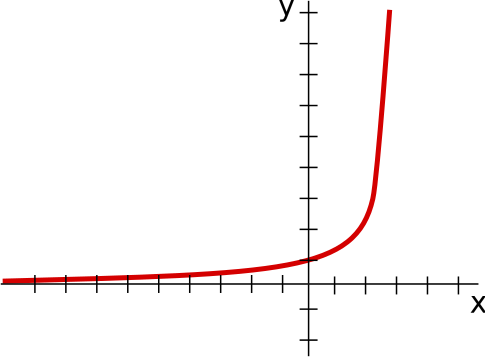
\includegraphics[width=2.5in]{images/exp2}$$

\begin{formulabox}[Three Types of Exponential Functions]
There are \ifont{three kinds} of exponential functions $f(x)=a^x$ depending on whether $a>1$, $a=1$ or $0<a<1$:
$$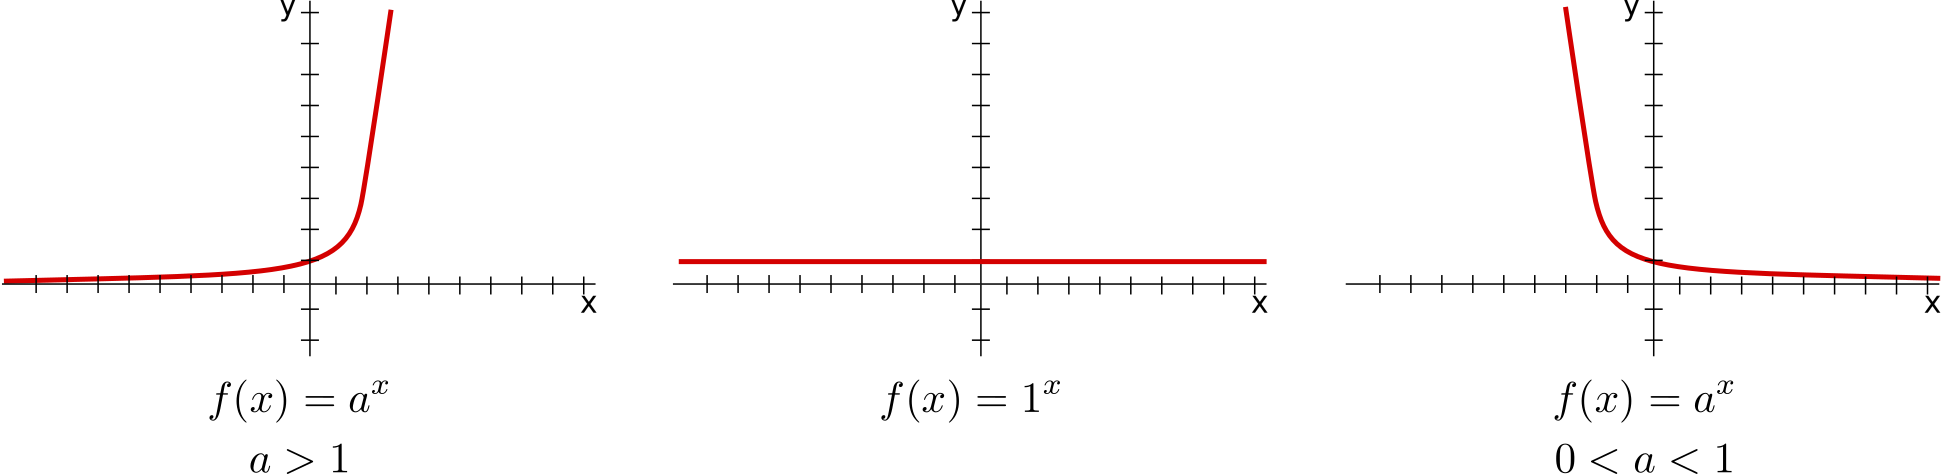
\includegraphics[width=6in]{images/exp3}$$
\end{formulabox}
 
\subsection*{Properties of Exponential Functions}
The first thing to note is that if $a<0$ then problems can occur.
Observe that if $a=-1$ then $(-1)^x$ is not defined for every $x$.
For example, $x=1/2$ is a square root and gives $(-1)^{1/2}=\sqrt{-1}$ which is not a real number.

\begin{formulabox}[Exponential Function Properties]
\begin{itemize}
\item \ifont{Only defined for positive $a$:} $a^x$ is only defined for all real $x$ if $a>0$
\item \ifont{Always positive:} $a^x>0$, for all $x$
\item \ifont{Exponent rules: }
\begin{multicols}{2}
\begin{enumerate}
	\item $\ds{a^xa^y=a^{x+y}}$
	\item $\ds{\frac{a^x}{a^y}=a^{x-y}}$
	\item $\ds{\left(a^x\right)^y=a^{xy}=a^{yx}=\left(a^y\right)^x}$
	\item $\ds{a^xb^x=(ab)^x}$
\end{enumerate}
\end{multicols}
\item \ifont{Long term behaviour:} If $a>1$, then $a^x\to\infty$ as $x\to\infty$ and $a^x\to 0$ as $x\to-\infty$.
\end{itemize}
\end{formulabox}

The last property can be observed from the graph. If $a>1$, then as $x$ gets larger and larger, so does $a^x$.
On the other hand, as $x$ gets large and negative, the function approaches the $x$-axis, that is, $a^x$ approaches $0$.

\begin{example}{Reflection of Exponential}{ReflectionExponential}
Determine an equation of the function after reflecting $y=2^x$ about the line $x=-2$.
\end{example}

\begin{solution} 
First reflect about the $y$-axis to get $y=2^{-x}$.
Now shift by $2\times 2=4$ units to the \ifont{left} to get $y=2^{-(x+4)}$.
Side note: Can you see why this sequence of transformations is the same as reflection in the line $x=-2$?
Can you come up with a general rule for these types of reflections?
\end{solution}

\begin{example}{Determine the Exponential Function}{DetermineExponentialFunction}
Determine the exponential function $f(x)=ka^x$ that passes through the points $(1,6)$ and $(2,18)$.
\end{example}

\begin{solution} 
We substitute our two points into the equation to get:
$$x=1,y=6\to6=ka^1$$
$$x=2,y=18\to18=ka^2$$
This gives us $6=ka$ and $18=ka^2$.
The first equation is $k=6/a$ and subbing this into the second gives: $18=(6/a)a^2$.
Thus, $18=6a$ and $a=3$.
Now we can see from $6=ka$ that $k=2$.
Therefore, the exponential function is $$f(x)=2\cdot 3^x.$$
%\vspace{-1cm}
\end{solution}

There is one base that is so important and convenient that we give it a special symbol.
This number is denoted by $e=2.71828\ldots$ (and is an irrational number). 
Its \ifont{importance} stems from the fact that it simplifies many formulas 
of Calculus and also shows up in other fields of mathematics.

\begin{example}{Domain of Function with Exponential}{DomainFunctionExponential}
Find the domain of $\ds f(x)=\frac{1}{\sqrt{e^x+1}}$.
\end{example}

\begin{solution} 
For domain, we cannot divide by zero or take the square root of negative numbers.
Note that one of the properties of exponentials is that they are always positive!
Thus, $e^x+1>0$ (in fact, as $e^x>0$ we actually have that $e^x+1$ is at least one).
Therefore, $e^x+1$ is never zero nor negative, and gives no restrictions on $x$.
Thus, the domain is $\R$.
\end{solution}


%%%%%%%%%%%%%%%%%%%%%%%%%%%%%%%%%%%%%%%%%%%%
\Opensolutionfile{solutions}[ex]
\section*{Exercises for \ref{sec:ExpFunctions}}

\begin{enumialphparenastyle}

%%%%%%%%%%
\begin{ex}
Determine an equation of the function $y=a^x$ passing through the point $(3,8)$.
\begin{sol}
$y=2^x$
\end{sol}
\end{ex}

%%%%%%%%%%
\begin{ex}
Find the $y$-intercept of $f(x)=4^x+6$.
\begin{sol}
$y=7$
\end{sol}
\end{ex}

%%%%%%%%%%
\begin{ex}
Find the $y$-intercept of $f(x)=2\left(\frac{1}{2}\right)^x$.
\begin{sol}
$y=2$
\end{sol}
\end{ex}

%%%%%%%%%%
\begin{ex}
Find the domain of $\ds{y=e^{-x}+e^{\frac{1}{x}}}$.
\begin{sol}
$x\neq 0$
\end{sol}
\end{ex}

\end{enumialphparenastyle}